% vim: set spell spelllang=es syntax=tex :

\section{Descripción del sistema de visión global para fútbol de robots físicos
sobre el que se basa la presente propuesta}

\sectionmark{Descripción del sistema de visión global para fútbol de robots...}

\label{descripcionSistemaBase}

El principal objetivo del sistema descripto en \cite{torres2014} es su
utilización como herramienta didáctica para la introducción a la visión por
computadora. El sistema define un framework de visión por computadora capaz de
adaptarse a distintos dominios, pero en el trabajo se ofrece una solución
específica para el fútbol de robots de la liga de tamaño pequeño.

El sistema está basado en pilas de plugins y utiliza múltiples hilos para
aprovechar hasta cuatro núcleos (para el fútbol de robots); pero si la
plataforma posee más núcleos, no serán utilizados. Cada uno de los hilos tiene
una responsabilidad diferente. El framework general tiene tres componentes
principales:

\begin{description}

	\item[Hilo principal:] es el hilo encargado de la interfaz gráfica de
		usuario.

	\item[Hilo de captura de cuadros:] es el hilo encargado de la captura o
		generación de los cuadros a partir de una cámara o archivo. El
		hilo de captura está desacoplado de los hilos de búsqueda o
		procesamiento de cuadros.

	\item[Hilos de procesamiento de cuadros:] estos hilos están formados por
		una pila de plugins que procesarán cada cuadro en forma
		secuencial. Normalmente, por cada tipo de objeto a reconocer,
		hay un hilo de este tipo dedicado a su detección. La diferencia
		entre ellos está en los plugins que componen la pila y en su
		orden. Existen mecanismos de control para asegurar que, si un
		cuadro es procesado por un hilo de procesamiento, entonces
		también será procesado por el resto de los hilos de
		procesamiento, asegurando al mismo tiempo que cada cuadro será
		procesado sólo una vez por cada hilo.

\end{description}

En la implementación de la solución específica para el fútbol de robots de la
\emph{SSL}, se crean dos hilos de procesamiento de cuadros, uno para la búsqueda
de los robots y el otro para la búsqueda de la pelota. Las primeras etapas de
procesamiento son iguales en ambos. Los primeros plugins son los de conversión
de color, segmentación de color y morfología. El hilo de procesamiento que busca
la pelota continúa con el plugin de búsqueda de pelota, mientras que aquél
encargado de la búsqueda de robots continúa con los plugins de detección de
regiones principales y detección de regiones secundarias. Ambos terminan con el
plugin de difusión. En la figura \ref{pilasPlugins} se muestran ambas pilas y
los plugins que las componen.

\begin{figure}[h]

	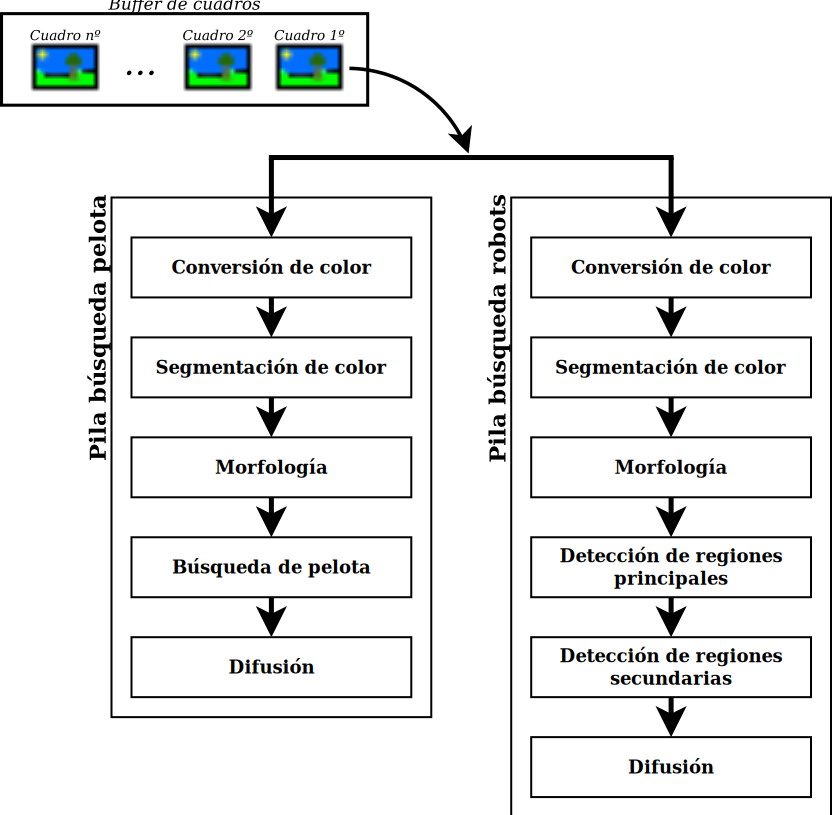
\includegraphics[width=\textwidth]{img/pilas.pdf}

	\caption{Pilas de plugins del sistema propuesto en \cite{torres2014}.}

	\label{pilasPlugins}

\end{figure}


De acuerdo a su función, los plugins pueden ser agrupados por las etapas de la
visión por computadora que implementan:

\begin{description}

	\item[Adquisición de la imagen:] Esta etapa está a cargo del hilo de
		captura de cuadros.

	\item[Preprocesamiento:] plugins de conversión de color, de segmentación
		de color y de morfología.

	\item[Extracción de características, Detección y Segmentación:] plugins
		de detección de regiones principales.

	\item[Procesamiento de alto nivel:] plugins de detección de pelota y de
		detección de regiones secundarias.

	\item[Toma de decisiones:] Dado que el sistema de visión para fútbol de
		robots no realiza toma de decisiones, el estado de la cancha es
		comunicado a las computadoras de los equipos a través del plugin
		de difusión.

\end{description}

El tiempo de generación de cuadros es fijo (o a demanda), mientras que el de
procesamiento es variable, pudiendo variar entre mayor que el tiempo de
generación o menor a éste. Por ello, cuando se genera un nuevo cuadro, éste se
coloca en un buffer. Si la capacidad de procesamiento es insuficiente, y no
hay más espacio en el buffer para almacenar un nuevo cuadro, se descarta el
cuadro más viejo. Esta estrategia da mayor prioridad a la información más
actual.

